Хранилище представляет собой импровизированное key-value хранилище, выбор среди
альтернатив которого, описан в REF.

Данные, которыми располагает приложение, подразумевают внесение изменений лишь
разработчиком приложения. Этими данными являются ссылки на сетевые адреса
хранения исходных кодов алгоритмов, пути записи алгоритмов в ФС компьютера, и
пути до функций-обёрток данных алгоритмов. Все представленные данные, при
необходимости, правятся разработчиком, в следствие чего, хранилище имеет только
метод \textbf{get} (Листинг \ref{lst:get}), и является read-only. Entity-relationship диаграмма
представлена на рисунке \ref{er}.

\begin{figure}[h]
    \centering
    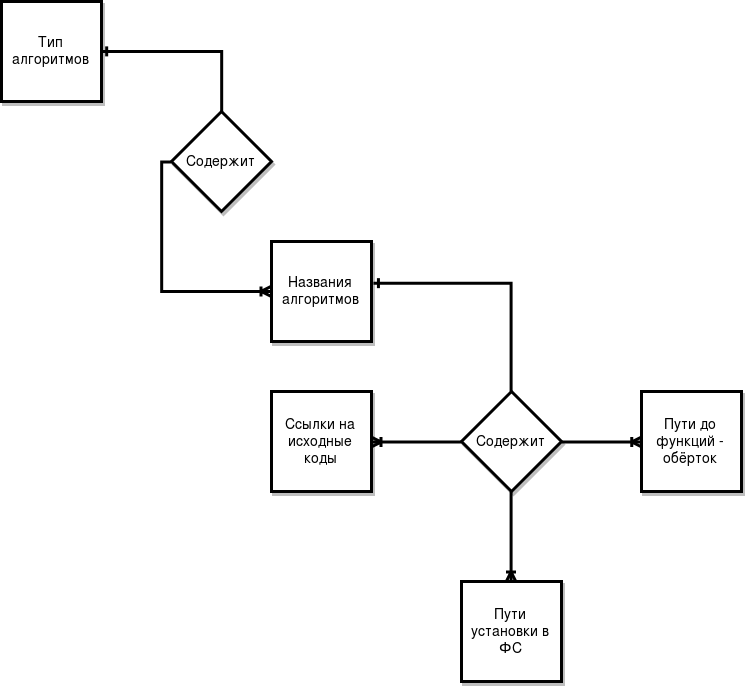
\includegraphics[width=\textwidth]{images/er}
    \caption{Диаграмма отношений сущностей в реализованном хранилище}\label{er}
\end{figure}

\newpage
Метод \textbf{get} хранилища:

\begin{center}
\begin{lstlisting}
def get(name, val, default=None):
    return getattr(_kv_, name).get(val, default)
\end{lstlisting}\label{lst:get}
Листинг \ref{lst:get}: код метода get хранилища
\end{center}

Код класса хранилища:
\begin{center}
\begin{lstlisting}
class _kv_(object):
    OPTIONS = {
            'hashing':  ['SHA-256', 'SHA-512', 'Scrypt', 'KECCAK-256',
                         'KECCAK-512', 'Ethash', 'X11', 'X17', 'myr-groestl',
                         'Lyra2rev2', 'blake2s', 'blake2b'],
#...                    
    }

    LINKS = { } # ....

    UPDATE_LINKS = { } # ....

    TOINSTALL = { } # ....

    INTERFACES = { } # ....
    \end{lstlisting}\label{lst:hran}
    Листинг \ref{lst:hran}: Представление кода реализованного key-value хранилища
\end{center}


